\documentclass[10pt,aspectratio=169]{beamer}

\usepackage[utf8]{inputenc}
\usepackage[T1]{fontenc}
\usepackage{tikz}
\usetikzlibrary{arrows.meta, positioning, fit, backgrounds, shapes.multipart}
\usepackage{booktabs}
\usepackage{array}
\usepackage{multirow}
\usepackage{xcolor}
\usepackage{tabularx}
\usepackage{hyperref}

\usetheme{Madrid}
\usecolortheme{seahorse}
\setbeamertemplate{navigation symbols}{}
\setbeamertemplate{footline}[frame number]
\setbeamercovered{transparent}

\definecolor{mblue}{RGB}{31,78,121}
\definecolor{morange}{RGB}{237,125,49}
\definecolor{mgreen}{RGB}{84,130,53}
\definecolor{mgray}{RGB}{89,89,89}
\definecolor{mpurple}{RGB}{112,48,160}

\setbeamercolor{structure}{fg=mblue}
\setbeamercolor{block title}{bg=mblue!15,fg=mblue}
\setbeamercolor{block body}{bg=mblue!5}

\newcommand{\pbox}[3]{
  % #1 = node name, #2 = color, #3 = text
  \node[draw=#2, thick, fill=#2!12, rounded corners, minimum height=1.1cm,
        text width=2.5cm, align=center, font=\scriptsize] (#1) {#3};
}

\title[Maquette $\to$ Modèle hiérarchique]{Analyse des méthodes de transformation d'une maquette en modèle hiérarchique pour la génération de code frontend}
\subtitle{Étude comparative : ScreenCoder, DesignCoder, Prototype2Code, DCGen, ReverseORC}
\author{Présentation à l'encadrant}
\date{\today}

\begin{document}

% ---------------------------------------------------------------
\begin{frame}
\titlepage
\end{frame}

% ---------------------------------------------------------------
\begin{frame}{Plan}
\tableofcontents
\end{frame}

% =================================================================
\section{Problématique}
% =================================================================
\begin{frame}{Problématique de recherche}
\begin{block}{Objectif}
Transformer automatiquement une \textbf{maquette d'interface} en une \textbf{représentation structurée / hiérarchique}, servant d'étape intermédiaire avant la génération de code frontend.
\end{block}

\begin{center}
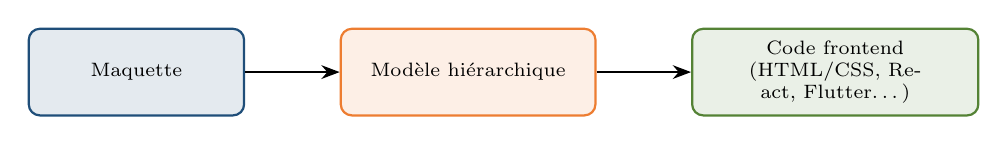
\begin{tikzpicture}[node distance=1.2cm, >=Stealth]
\pbox{a}{mblue}{Maquette}
\node[draw=morange, thick, fill=morange!12, rounded corners, minimum height=1.1cm,
      text width=3cm, align=center, font=\scriptsize, right=1.2cm of a] (b) {Modèle hiérarchique};
\node[draw=mgreen, thick, fill=mgreen!12, rounded corners, minimum height=1.1cm,
      text width=3.4cm, align=center, font=\scriptsize, right=1.2cm of b] (c) {Code frontend (HTML/CSS, React, Flutter\ldots)};
\draw[-{Stealth},thick] (a) -- (b);
\draw[-{Stealth},thick] (b) -- (c);
\end{tikzpicture}
\end{center}

\vspace{2mm}
\textbf{Question centrale : } comment chaque méthode passe-t-elle de la maquette à sa représentation structurée ?
\end{frame}

\begin{frame}{Grille d'analyse utilisée}
Pour chaque méthode étudiée, on cherche à identifier :
\begin{itemize}
  \item les \textbf{données en entrée} (image seule ? métadonnées de design ? plusieurs tailles ?)
  \item la \textbf{façon d'analyser} la maquette (règles, MLLM, accessibilité API\ldots)
  \item les \textbf{éléments détectés/extraits} et les informations associées
  \item la \textbf{détermination des relations} (parent-enfant, alignement, groupement)
  \item la \textbf{méthode de construction} du modèle (règles déterministes vs génératif)
  \item la \textbf{forme finale} du modèle (arbre ? DOM-like ? contraintes OR ?)
  \item les \textbf{étapes intermédiaires}
  \item l'\textbf{usage en aval} pour générer le code
\end{itemize}
\end{frame}

% =================================================================
\section{ScreenCoder}
% =================================================================
\begin{frame}{ScreenCoder --- vue d'ensemble}
\footnotesize Jiang et al., \emph{ScreenCoder: Advancing Visual-to-Code Generation for Front-End Automation via Modular Multimodal Agents}, 2025.

\vspace{2mm}
\textbf{Idée clé} : décomposer la tâche en 3 agents spécialisés pour corriger les erreurs de \emph{perception} et de \emph{planification} des MLLM monolithiques.

\begin{center}
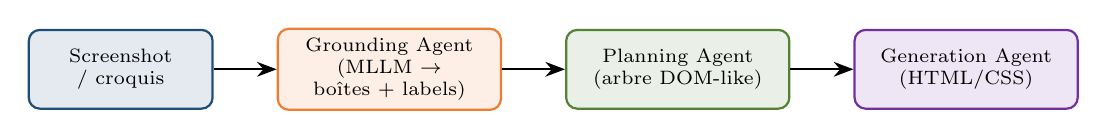
\begin{tikzpicture}[node distance=8mm and 8mm, >=Stealth]
\node[draw=mblue,thick,fill=mblue!12,rounded corners,text width=2.1cm,align=center,minimum height=1cm,font=\scriptsize] (a) {Screenshot / croquis};
\node[draw=morange,thick,fill=morange!12,rounded corners,text width=2.6cm,align=center,minimum height=1cm,font=\scriptsize, right=of a] (b) {Grounding Agent\\(MLLM $\to$ boîtes + labels)};
\node[draw=mgreen,thick,fill=mgreen!12,rounded corners,text width=2.6cm,align=center,minimum height=1cm,font=\scriptsize, right=of b] (c) {Planning Agent\\(arbre DOM-like)};
\node[draw=mpurple,thick,fill=mpurple!12,rounded corners,text width=2.6cm,align=center,minimum height=1cm,font=\scriptsize, right=of c] (d) {Generation Agent\\(HTML/CSS)};
\draw[-{Stealth[length=2.5mm]},thick] (a) -- (b);
\draw[-{Stealth[length=2.5mm]},thick] (b) -- (c);
\draw[-{Stealth[length=2.5mm]},thick] (c) -- (d);
\end{tikzpicture}
\end{center}
\end{frame}

\begin{frame}{ScreenCoder --- Grounding Agent}
\textbf{Entrée :} image (screenshot ou croquis) uniquement.

\textbf{Méthode :} MLLM interrogé par des prompts type \emph{``Where is the sidebar?''} $\Rightarrow$ ensemble
$$\mathcal{B} = \{(b_i,l_i)\mid l_i \in \mathcal{L}\}, \quad \mathcal{L}=\{\text{sidebar, header, navigation}, \ldots\}$$

\textbf{Post-traitement (robustesse) :}
\begin{itemize}
  \item \textbf{Déduplication / NMS} par classe pour éliminer les détections redondantes
  \item \textbf{Fallback heuristique} si un composant clé manque (ex. boîte large et basse en haut $\to$ header)
  \item \textbf{Inférence du contenu principal} = plus grande zone rectangulaire non couverte
\end{itemize}

\textbf{Sortie :} un \emph{dictionnaire de layout} (labels + boîtes) $\to$ fondation sémantique/spatiale.
\end{frame}

\begin{frame}{ScreenCoder --- Planning Agent (Algorithme 1)}
\textbf{Approche déterministe} (pas générative) : \emph{Visual-to-Structural Tree Mapping}.

\begin{block}{Principe}
\begin{enumerate}
  \item Créer un n\oe ud racine + un n\oe ud par composant primaire (header, sidebar\ldots)
  \item Convertir coordonnées pixel $\to$ pourcentages responsives
  \item Positionnement \texttt{absolute} pour préserver la macro-structure
  \item Marquer les régions à enfants multiples comme conteneurs \texttt{CSS Grid}
\end{enumerate}
\end{block}

\textbf{Forme du modèle :} arbre DOM-like, avec styles \texttt{position:absolute} + \texttt{grid} imbriqués.
\textbf{Avantage revendiqué :} fidélité structurelle et prévisibilité (au prix de la flexibilité générative).
\end{frame}

\begin{frame}{ScreenCoder --- Génération et Placeholder Mapping}
\textbf{Generation Agent :} parcourt l'arbre, génère HTML/CSS par n\oe ud via prompt adaptatif (label sémantique + contexte structurel + instructions utilisateur optionnelles) $\to$ assemblage selon la hiérarchie.

\textbf{Placeholder mapping (étape finale) :}
\begin{itemize}
  \item Détection des visuels réels (UIED) dans le screenshot source
  \item Partition par région sémantique (header, sidebar\ldots)
  \item Appariement optimal \emph{placeholders} $\leftrightarrow$ éléments réels (coût = $-$CIoU, résolu par \textbf{algorithme hongrois})
  \item Insertion des images recadrées dans le code généré
\end{itemize}
\textbf{Sert aussi de moteur de données} : génère Screen-10K (10k paires image-code) pour fine-tuner un MLLM (SFT + RL avec récompense $-$MSE pixel).
\end{frame}

% =================================================================
\section{DesignCoder}
% =================================================================
\begin{frame}{DesignCoder --- vue d'ensemble}
\footnotesize Chen et al., \emph{DesignCoder: Hierarchy-Aware and Self-Correcting UI Code Generation with LLMs}, 2025.

\vspace{2mm}
\textbf{Différence majeure :} entrée = \textbf{maquette Figma/Sketch} (image \emph{+ métadonnées de design} : id, bbox, type, style) et non un simple screenshot brut.

\begin{center}
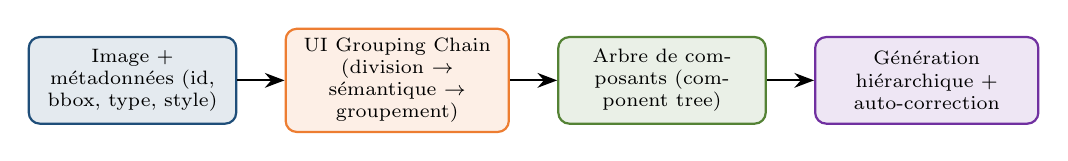
\begin{tikzpicture}[node distance=8mm and 6mm, >=Stealth]
\node[draw=mblue,thick,fill=mblue!12,rounded corners,text width=2.4cm,align=center,minimum height=1.1cm,font=\scriptsize] (a) {Image + métadonnées (id, bbox, type, style)};
\node[draw=morange,thick,fill=morange!12,rounded corners,text width=2.6cm,align=center,minimum height=1.1cm,font=\scriptsize, right=of a] (b) {UI Grouping Chain\\(division $\to$ sémantique $\to$ groupement)};
\node[draw=mgreen,thick,fill=mgreen!12,rounded corners,text width=2.4cm,align=center,minimum height=1.1cm,font=\scriptsize, right=of b] (c) {Arbre de composants (component tree)};
\node[draw=mpurple,thick,fill=mpurple!12,rounded corners,text width=2.6cm,align=center,minimum height=1.1cm,font=\scriptsize, right=of c] (d) {Génération hiérarchique + auto-correction};
\draw[-{Stealth[length=2.5mm]},thick] (a) -- (b);
\draw[-{Stealth[length=2.5mm]},thick] (b) -- (c);
\draw[-{Stealth[length=2.5mm]},thick] (c) -- (d);
\end{tikzpicture}
\end{center}
\end{frame}

\begin{frame}{DesignCoder --- UI Grouping Chain (3 sous-tâches)}
\begin{enumerate}
  \item \textbf{Division (UI division)} : un LLM segmente la liste de couches $L_{layers}$ (id, bbox, type) en sous-régions sémantiques $D$, avec correction algorithmique (Alg. 1) : fusion des régions qui se chevauchent, réassignation des couches orphelines à la région la plus proche, borne 3--10 régions.
  \item \textbf{Extraction sémantique} : pour chaque sous-région, un MLLM décrit chaque élément (fonction, relations) à partir de l'image recadrée + métadonnées $\to$ $L_{semantic}$.
  \item \textbf{Groupement (Grouping)} : un prompt structuré organise $L_{semantic}$ en \textbf{arbre hiérarchique de composants}, avec post-traitement anti-chevauchement / anti-n\oe uds parasites.
\end{enumerate}
\textbf{Forme du modèle :} arbre de composants \emph{sémantiques} (pas seulement géométriques), chaque n\oe ud portant une description fonctionnelle.
\end{frame}

\begin{frame}{DesignCoder --- Génération et auto-correction}
\textbf{Génération de code (divide-and-conquer) :}
\begin{itemize}
  \item Code composant : LLM ``expert React'' suit strictement l'arbre, assigne des identifiants de composants
  \item Style CSS : parcours de l'arbre \emph{bottom-up} ; feuilles gardent leurs bbox, n\oe uds internes agrègent les bbox enfants (taille/position relative)
\end{itemize}

\textbf{Self-correcting refinement (spécificité forte) :}
\begin{itemize}
  \item Rendu réel (Appium) $\to$ comparaison image par image, composant par composant (\emph{visual analysis prompt})
  \item Génération de suggestions de correction $\to$ réparation ciblée et parallélisable par composant
  \item Boucle possible tant que des différences visuelles subsistent
\end{itemize}
\textbf{Point clé :} le modèle hiérarchique n'est pas figé après construction — il est \emph{revisité} via une boucle de vérification visuelle.
\end{frame}

% =================================================================
\section{Prototype2Code}
% =================================================================
\begin{frame}{Prototype2Code --- vue d'ensemble}
\footnotesize Xiao et al., \emph{Prototype2code: End-to-end front-end code generation from UI design prototypes}, 2024 (méthode également utilisée comme baseline par ScreenCoder \& DesignCoder).

\vspace{2mm}
\textbf{Approche : purement à base de règles} (pas de génération par LLM pour la structure) — construction \textbf{déterministe} d'un arbre ``poupée russe'' puis segmentation Flexbox.

\begin{center}
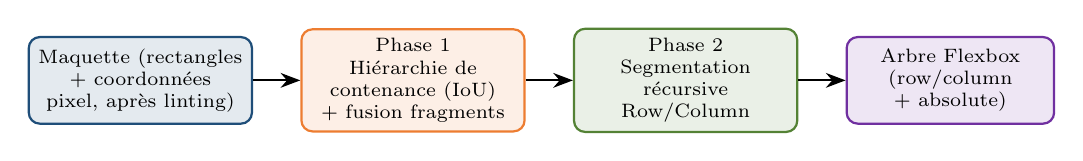
\begin{tikzpicture}[node distance=8mm and 6mm, >=Stealth]
\node[draw=mblue,thick,fill=mblue!12,rounded corners,text width=2.6cm,align=center,minimum height=1.1cm,font=\scriptsize] (a) {Maquette (rectangles + coordonnées pixel, après linting)};
\node[draw=morange,thick,fill=morange!12,rounded corners,text width=2.6cm,align=center,minimum height=1.1cm,font=\scriptsize, right=of a] (b) {Phase 1\\Hiérarchie de contenance (IoU) + fusion fragments};
\node[draw=mgreen,thick,fill=mgreen!12,rounded corners,text width=2.6cm,align=center,minimum height=1.1cm,font=\scriptsize, right=of b] (c) {Phase 2\\Segmentation récursive Row/Column};
\node[draw=mpurple,thick,fill=mpurple!12,rounded corners,text width=2.4cm,align=center,minimum height=1.1cm,font=\scriptsize, right=of c] (d) {Arbre Flexbox (row/column + absolute)};
\draw[-{Stealth[length=2.5mm]},thick] (a) -- (b);
\draw[-{Stealth[length=2.5mm]},thick] (b) -- (c);
\draw[-{Stealth[length=2.5mm]},thick] (c) -- (d);
\end{tikzpicture}
\end{center}
\end{frame}

\begin{frame}{Prototype2Code --- Phase 1 : hiérarchie de contenance}
\begin{enumerate}
  \item Tri des groupes perceptuels (cartes, barres\ldots) par taille \textbf{croissante}
  \item Calcul d'\textbf{IoU} pour rattacher chaque couche à son groupe géométrique
  \item \textbf{Fusion} des éléments fragmentés (ex. icône coupée) en une seule entité
  \item Insertion des feuilles (triées par taille \textbf{décroissante}) sous le n\oe ud le plus petit qui les contient $\to$ structure ``poupée russe''
  \item Si des enfants d'un n\oe ud se chevauchent $\Rightarrow$ nouveau parent avec \texttt{need\_absolute=True} (positionnement CSS absolu)
\end{enumerate}
\textbf{Caractère :} entièrement géométrique / à base de règles (pas de compréhension sémantique du contenu).
\end{frame}

\begin{frame}{Prototype2Code --- Phase 2 : segmentation Flexbox}
\begin{enumerate}
  \item \textbf{Segmentation verticale} : recherche de coordonnées $Y$ traversant la zone sans couper d'élément $\to$ ``étages''
  \item \textbf{Segmentation horizontale} : à l'intérieur de chaque étage, recherche de coordonnées $X$ $\to$ colonnes
  \item \textbf{Récursion} jusqu'à impossibilité de segmenter davantage
  \item Attribution de \texttt{flex-direction: row} ou \texttt{column} selon l'alignement détecté
\end{enumerate}

\textbf{Forme finale :} arbre où chaque n\oe ud porte une instruction de mise en page explicite (Flexbox row/column, ou absolute) $\to$ mappage quasi direct vers HTML imbriqué + CSS.
\end{frame}

% =================================================================
\section{DCGen}
% =================================================================
\begin{frame}{DCGen (Divide-and-Conquer) --- vue d'ensemble}
\footnotesize Wan et al., \emph{Divide-and-Conquer: Generating UI Code from Screenshots}, FSE 2025.

\vspace{2mm}
\textbf{Constat (étude de motivation) :} un MLLM appliqué directement produit 3 types d'erreurs — \emph{omission}, \emph{distorsion}, \emph{mauvais agencement} d'éléments (85\,\% omission dans leur étude). Recadrer l'image en segments plus petits améliore nettement la qualité (similarité CLIP 73,7\,\%$\to$76,0\,\%).

\begin{center}
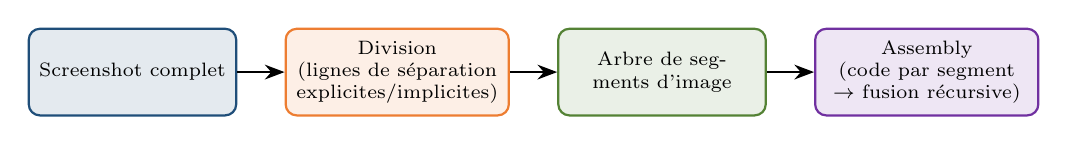
\begin{tikzpicture}[node distance=8mm and 6mm, >=Stealth]
\node[draw=mblue,thick,fill=mblue!12,rounded corners,text width=2.4cm,align=center,minimum height=1.1cm,font=\scriptsize] (a) {Screenshot complet};
\node[draw=morange,thick,fill=morange!12,rounded corners,text width=2.6cm,align=center,minimum height=1.1cm,font=\scriptsize, right=of a] (b) {Division\\(lignes de séparation explicites/implicites)};
\node[draw=mgreen,thick,fill=mgreen!12,rounded corners,text width=2.4cm,align=center,minimum height=1.1cm,font=\scriptsize, right=of b] (c) {Arbre de segments d'image};
\node[draw=mpurple,thick,fill=mpurple!12,rounded corners,text width=2.6cm,align=center,minimum height=1.1cm,font=\scriptsize, right=of c] (d) {Assembly\\(code par segment $\to$ fusion récursive)};
\draw[-{Stealth[length=2.5mm]},thick] (a) -- (b);
\draw[-{Stealth[length=2.5mm]},thick] (b) -- (c);
\draw[-{Stealth[length=2.5mm]},thick] (c) -- (d);
\end{tikzpicture}
\end{center}
\end{frame}

\begin{frame}{DCGen --- Division : détection de lignes de séparation}
\textbf{Particularité :} pas de détection d'éléments UI typés (pas de ``sidebar/header''!) — on détecte des \textbf{lignes de coupure géométriques} dans l'image brute (niveaux de gris).

\begin{itemize}
  \item \textbf{Lignes explicites} : bordures visibles (changement brutal de pixels)
  \item \textbf{Lignes implicites} : zones de faible variance (espaces blancs) encadrées par des transitions de luminosité (fenêtre glissante, double seuillage \texttt{var\_thr}/\texttt{diff\_thr})
  \item Division \textbf{alterné et récursif} horizontal $\to$ vertical, jusqu'à profondeur max ou absence de nouvelle ligne
\end{itemize}

\textbf{Forme du modèle intermédiaire :} arbre de subdivisions \emph{purement géométrique} (pas de sémantique de composants), chaque n\oe ud = un segment d'image.
\end{frame}

\begin{frame}{DCGen --- Assembly : reconstruction du code}
Deux variantes proposées :
\begin{columns}
\begin{column}{0.5\textwidth}
\textbf{Agent-based}
\begin{itemize}
  \item MLLM ``leaf-solver'' génère le code de chaque feuille
  \item MLLM ``assembly'' fusionne récursivement enfants $\to$ parent
  \item MLLM ``generation'' produit le code final (racine)
\end{itemize}
\end{column}
\begin{column}{0.5\textwidth}
\textbf{Rule-based}
\begin{itemize}
  \item Génération de code \emph{uniquement} au niveau des feuilles
  \item Positionnement automatique via \textbf{CSS Grid} selon les positions enregistrées des segments
  \item Un LLM final ajuste la cohésion
\end{itemize}
\end{column}
\end{columns}
\vspace{2mm}
\textbf{Bilan :} pas de modèle sémantique hiérarchique construit explicitement — la hiérarchie est \emph{géométrique} (arbre de coupes), et sert de guide de \emph{prompting} plutôt que de structure de sortie interprétable.
\end{frame}

% =================================================================
\section{ReverseORC}
% =================================================================
\begin{frame}{ReverseORC --- vue d'ensemble}
\footnotesize Jiang, Stuerzlinger, Lutteroth, \emph{ReverseORC: Reverse Engineering of Resizable UI Layouts with OR-Constraints}, CHI 2021.

\vspace{2mm}
\alert{Particularité majeure : ce n'est pas un pipeline maquette-unique $\to$ code.} L'entrée est un ensemble d'\textbf{échantillons du même UI à plusieurs tailles de fenêtre}, obtenus via API d'accessibilité (pas une image).

\begin{center}
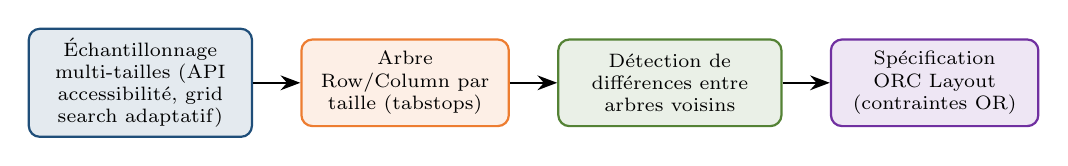
\begin{tikzpicture}[node distance=8mm and 6mm, >=Stealth]
\node[draw=mblue,thick,fill=mblue!12,rounded corners,text width=2.6cm,align=center,minimum height=1.1cm,font=\scriptsize] (a) {Échantillonnage multi-tailles (API accessibilité, grid search adaptatif)};
\node[draw=morange,thick,fill=morange!12,rounded corners,text width=2.4cm,align=center,minimum height=1.1cm,font=\scriptsize, right=of a] (b) {Arbre Row/Column par taille (tabstops)};
\node[draw=mgreen,thick,fill=mgreen!12,rounded corners,text width=2.6cm,align=center,minimum height=1.1cm,font=\scriptsize, right=of b] (c) {Détection de différences entre arbres voisins};
\node[draw=mpurple,thick,fill=mpurple!12,rounded corners,text width=2.4cm,align=center,minimum height=1.1cm,font=\scriptsize, right=of c] (d) {Spécification ORC Layout (contraintes OR)};
\draw[-{Stealth[length=2.5mm]},thick] (a) -- (b);
\draw[-{Stealth[length=2.5mm]},thick] (b) -- (c);
\draw[-{Stealth[length=2.5mm]},thick] (c) -- (d);
\end{tikzpicture}
\end{center}
\end{frame}

\begin{frame}{ReverseORC --- Construction de l'arbre par taille}
\textbf{Extraction :} API d'accessibilité $\to$ id, taille, position (top-left) de chaque widget (pas de reconnaissance d'image).

\textbf{Tabstops} : variables symboliques représentant les alignements (x-tabstop / y-tabstop). Un tabstop est un \textbf{layout divider} s'il coupe la maquette en deux sans traverser aucun widget.

\textbf{Reconstruction récursive (façon XY-Cut)} :
\begin{itemize}
  \item Deux widgets $\to$ même \emph{Row} s'ils sont entre les deux mêmes diviseurs horizontaux (idem \emph{Column})
  \item Subdivision horizontale prioritaire, puis verticale, sinon tabstops seuls (cas rare, ex. pinwheel)
  \item Regroupement de sous-couches consécutives si cela simplifie la structure
\end{itemize}
\textbf{Forme :} arbre Row/Column (comme Prototype2Code) mais recalculé \textbf{indépendamment à chaque taille échantillonnée}.
\end{frame}

\begin{frame}{ReverseORC --- Diff. d'arbres $\to$ patterns ORC}
\textbf{Détection de différences} entre arbres de tailles voisines (édition d'arbres avec identités partielles) : \texttt{addNode}, \texttt{removeNode}, \texttt{moveNode}, \texttt{replaceNode}, \texttt{changeType}, \texttt{changeChildrenOrder}.

\textbf{Mapping règle $\to$ pattern ORC} (contrainte disjonctive ``\emph{A OU B}'') :
\begin{itemize}
  \item \texttt{removeNode} (feuille) $\to$ \textbf{widget optionnel}
  \item \texttt{moveNode} (enfants consécutifs) $\to$ fusion en \textbf{flux horizontal/vertical} ; sinon \textbf{position alternative}
  \item \texttt{replaceNode} $\to$ \textbf{layout alternatif}
  \item \texttt{changeType} $\to$ \textbf{sous-layout pivot} (Row $\leftrightarrow$ Column)
\end{itemize}
\textbf{Sortie finale :} une \textbf{unique spécification ORC Layout}, valable sur \emph{toute la plage de tailles}, avec une \emph{error map} visualisant la fidélité de reconstruction (erreur structurelle, de transition, ``fault lines'').
\end{frame}

% =================================================================
\section{Comparaison}
% =================================================================
\begin{frame}{Différences clés entre les méthodes}
\begin{itemize}
  \item \textbf{Règles vs apprentissage} : Prototype2Code, DCGen(division) et ReverseORC sont \emph{déterministes / à base de règles} ; ScreenCoder (planning) est aussi déterministe mais le \emph{grounding} utilise un MLLM ; DesignCoder utilise un LLM à \emph{chaque} sous-étape.
  \item \textbf{Image seule vs métadonnées} : ScreenCoder \& DCGen travaillent sur l'\emph{image seule} ; DesignCoder \& Prototype2Code exploitent des \emph{métadonnées de design} (bbox/type/style) ; ReverseORC n'utilise \emph{aucune image}, seulement les propriétés de widgets via API.
  \item \textbf{Détection d'abord vs hiérarchie directe} : ScreenCoder détecte des \emph{régions labellisées} puis construit l'arbre ; Prototype2Code/ReverseORC/DCGen \emph{ne labellisent pas} sémantiquement, ils coupent géométriquement l'espace.
  \item \textbf{Relations parent-enfant} : via \emph{IoU} + inclusion (Prototype2Code), via \emph{tabstops/layout dividers} (ReverseORC), via \emph{lignes de séparation par variance} (DCGen), via \emph{prompt de groupement sémantique} (DesignCoder), via \emph{position absolue + grid} (ScreenCoder).
  \item \textbf{Nature du modèle final} : arbre \emph{géométrique} pur (Prototype2Code, DCGen, ReverseORC) vs arbre \emph{sémantique} enrichi (DesignCoder) vs arbre \emph{DOM-like stylé} (ScreenCoder) vs \emph{contraintes OR multi-tailles} (ReverseORC, unique dans ce corpus).
\end{itemize}
\end{frame}

\begin{frame}{Similitudes entre les méthodes}
\begin{itemize}
  \item Toutes convergent vers une structure \textbf{arborescente récursive de type conteneur} (Row/Column, Grid, ou arbre DOM) : le \emph{modèle hiérarchique} est un invariant conceptuel du domaine.
  \item Toutes (sauf ReverseORC) partent d'une \textbf{unique image/maquette statique}.
  \item Plusieurs méthodes (ScreenCoder, Prototype2Code, DCGen) séparent explicitement \textbf{détection/segmentation} et \textbf{génération de code}, illustrant un principe de \emph{separation of concerns}.
  \item La \textbf{gestion des chevauchements} est un problème récurrent, résolu soit par positionnement absolu (Prototype2Code, ScreenCoder), soit par contraintes OR (ReverseORC).
  \item Plusieurs méthodes (ScreenCoder, DesignCoder, DCGen) exploitent un \textbf{découpage en sous-problèmes plus petits} pour pallier les limites de perception/planification des MLLM (\emph{divide-and-conquer}).
\end{itemize}
\end{frame}

\begin{frame}{Tableau comparatif global (1/2)}
\centering
\renewcommand{\arraystretch}{1.3}
\resizebox{\textwidth}{!}{%
\begin{tabular}{l p{2.6cm} p{2.6cm} p{2.6cm} p{2.6cm} p{2.6cm}}
\toprule
\textbf{Critère} & \textbf{ScreenCoder} & \textbf{DesignCoder} & \textbf{Prototype2Code} & \textbf{DCGen} & \textbf{ReverseORC} \\
\midrule
Entrée & Screenshot / croquis (image seule) & Maquette Figma/Sketch + métadonnées & Maquette + métadonnées (post-linting) & Screenshot (image seule) & Widgets à $N$ tailles (API accessibilité, pas d'image) \\
Analyse maquette & MLLM (grounding par prompts) & LLM (division sémantique) & Règles géométriques (IoU) & Détection de lignes (variance pixel) & Extraction API + tabstops \\
Détection composants & Régions labellisées (sidebar, header\ldots) & Couches groupées sémantiquement & Groupes perceptuels fusionnés & Segments d'image non typés & Widgets individuels (typés par l'appli) \\
\bottomrule
\end{tabular}}
\end{frame}

\begin{frame}{Tableau comparatif global (2/2)}
\centering
\renewcommand{\arraystretch}{1.3}
\resizebox{\textwidth}{!}{%
\begin{tabular}{l p{2.6cm} p{2.6cm} p{2.6cm} p{2.6cm} p{2.6cm}}
\toprule
\textbf{Critère} & \textbf{ScreenCoder} & \textbf{DesignCoder} & \textbf{Prototype2Code} & \textbf{DCGen} & \textbf{ReverseORC} \\
\midrule
Relations & Position absolue + Grid & Groupement sémantique par LLM & IoU + inclusion géométrique & Lignes de séparation & Tabstops / layout dividers \\
Construction modèle & Déterministe (Alg.\,1) sur sortie MLLM & LLM (prompt de groupement) + post-traitement & Règles (Alg.\,1, poupée russe + Flexbox) & Récursion géométrique (XY-cut-like) & Récursion géométrique (XY-cut) $\times N$ tailles \\
Type de représentation & Arbre DOM-like stylé & Arbre de composants sémantiques & Arbre Row/Column Flexbox & Arbre de segments d'image & Arbre Row/Column $\to$ spéc.\ ORC (contraintes OR) \\
Génération code & Par n\oe ud + placeholder mapping (Hongrois) & Divide-and-conquer + auto-correction visuelle & Mapping direct vers Flexbox & Assembly agent/rule-based & Solveur ORC (multi-plateforme) \\
Avantages & Robuste aux erreurs de perception & Sémantique riche, auto-corrigé & Simple, rapide, interprétable & Réduit omissions/distorsions & Seule à capturer le \emph{redimensionnement} \\
Limites & Dépend du MLLM de grounding & Coût LLM élevé (plusieurs passes) & Pas de compréhension sémantique & Pas de sémantique de composant & Nécessite API accessibilité, pas d'image \\
\bottomrule
\end{tabular}}
\end{frame}

% =================================================================
\section{Mise en perspective}
% =================================================================
\begin{frame}{Constats pour ma problématique de recherche}
\begin{itemize}
  \item Le choix \textbf{image seule vs métadonnées} conditionne fortement la richesse du modèle : les métadonnées (DesignCoder, Prototype2Code) évitent les erreurs de perception mais supposent un accès au fichier de design (Figma/Sketch), non toujours disponible.
  \item Les approches \textbf{purement géométriques} (Prototype2Code, DCGen) donnent une structure \emph{correcte mais sans étiquette sémantique} — utile pour la mise en page, insuffisant pour un code maintenable/accessible.
  \item Les approches \textbf{hybrides} (ScreenCoder : grounding sémantique + construction déterministe de l'arbre) semblent offrir le meilleur compromis robustesse/interprétabilité.
  \item \textbf{ReverseORC} montre qu'un modèle hiérarchique statique est insuffisant si l'objectif inclut le \emph{comportement responsive} : il faudrait échantillonner ou raisonner sur plusieurs tailles, ou encoder des règles de flux (flow) directement dans le modèle.
  \item Les mécanismes d'\textbf{auto-correction visuelle} (DesignCoder) suggèrent qu'un modèle hiérarchique ne doit pas nécessairement être figé après une seule passe.
\end{itemize}
\end{frame}

\begin{frame}{Caractéristiques souhaitées pour le modèle hiérarchique visé}
\begin{enumerate}
  \item \textbf{Structure arborescente} générique (conteneurs Row/Column/Grid imbriqués), indépendante du framework cible (HTML/CSS, React, Flutter).
  \item \textbf{Étiquetage sémantique} des n\oe uds (rôle : header, navigation, card, liste\ldots), pas seulement géométrique.
  \item \textbf{Gestion explicite des cas ambigus} : chevauchement (positionnement absolu / z-index), éléments optionnels, alternatives de position.
  \item \textbf{Robustesse au bruit de détection} (fallback heuristiques comme ScreenCoder, ou vérification visuelle comme DesignCoder).
  \item \textbf{Possibilité (à terme) de capturer le redimensionnement} sans nécessiter un échantillonnage lourd multi-tailles (inspiration ReverseORC / OR-constraints, mais à partir d'une seule maquette si possible).
  \item \textbf{Traçabilité vers la génération multi-cible} : le modèle doit rester assez générique pour piloter plusieurs générateurs de code (HTML/CSS, React, Flutter) sans re-analyse de la maquette.
\end{enumerate}
\end{frame}

\begin{frame}{Synthèse}
\begin{block}{À retenir}
\begin{itemize}
  \item Toutes les méthodes convergent vers une \textbf{structure arborescente de conteneurs}, mais diffèrent radicalement sur \emph{comment} elles l'obtiennent (règles géométriques, MLLM, métadonnées, multi-échantillonnage).
  \item Le \textbf{compromis robustesse / richesse sémantique / coût} est le fil conducteur de la comparaison.
  \item ReverseORC introduit une dimension absente ailleurs : le \textbf{comportement dynamique} du layout.
\end{itemize}
\end{block}
\vspace{3mm}
\centering
\Large Prochaine étape : définir le modèle hiérarchique cible pour la génération multi-technologies.
\end{frame}

% =================================================================
\section{Bibliographie}
% =================================================================
\begin{frame}{Bibliographie}
\footnotesize
\begin{itemize}
  \item Jiang, Y., Zheng, Y., Wan, Y., Han, J., Wang, Q., Lyu, M.\,R., Yue, X. \emph{ScreenCoder: Advancing Visual-to-Code Generation for Front-End Automation via Modular Multimodal Agents.} arXiv:2507.22827, 2025. \url{https://arxiv.org/abs/2507.22827}
  \item Chen, Y., Ding, S., Zhang, Y., Chen, W., Du, J., Sun, L., Chen, L. \emph{DesignCoder: Hierarchy-Aware and Self-Correcting UI Code Generation with Large Language Models.} arXiv:2506.13663, 2025. \url{https://arxiv.org/abs/2506.13663}
  \item Xiao, S., Chen, Y., Li, J., Chen, L., Sun, L., Zhou, T. \emph{Prototype2code: End-to-end front-end code generation from UI design prototypes.} IDETC/CIE 2024.
  \item Wan, Y., Wang, C., Dong, Y., Wang, W., Li, S., Huo, Y., Lyu, M. \emph{Divide-and-Conquer: Generating UI Code from Screenshots.} Proc. ACM Softw. Eng. (FSE), 2025. \url{https://doi.org/10.1145/3729364}
  \item Jiang, Y., Stuerzlinger, W., Lutteroth, C. \emph{ReverseORC: Reverse Engineering of Resizable User Interface Layouts with OR-Constraints.} CHI 2021. \url{https://doi.org/10.1145/3411764.3445043}
\end{itemize}
\end{frame}

\begin{frame}
\centering
\Large Merci --- Questions ?
\end{frame}

\end{document}